\section{Problem Statement}
\label{sec:problem-statement}
    \lettrine[lines=2]{\scalebox{1.1}{\textbf{S}}}{TRING} matching is a problem that 
    find all occurrences of a pattern in the text.
    This problem is an indispensable technique in computer science for solving various crucial problems,
    such as text editing, text searching, and symbol manipulation.\cite{hakak2019exact}

    \indent The string matching problem is defined as follows:
    We assume that the text is a string $T[1..n]$ of length $n$ and the pattern is a string $P[1..m]$ of length $m$
    which $m \le n$. The problem is to find all occurrences of $P$ in $T$ by shifting $P$ along $T$ such that
    $0 \le s \le n-m$ ($s$ is the shift amount) and $T[s+1..s+m] = P[1..m]$ (that is, if $T[s+i]=P[i]$, for $1 \le i \le m$).\cite{cormen2022introduction}
    
    \indent \textbf{For instance:}
    \begin{itemize}
        \item If $T = \text{``ababcab''}$ and $P = \text{``abc''}$, then the output is $(3 \rightarrow 5)$ because the pattern occurs at position 3 in the text.
        \begin{figure}[h]
            \centering
            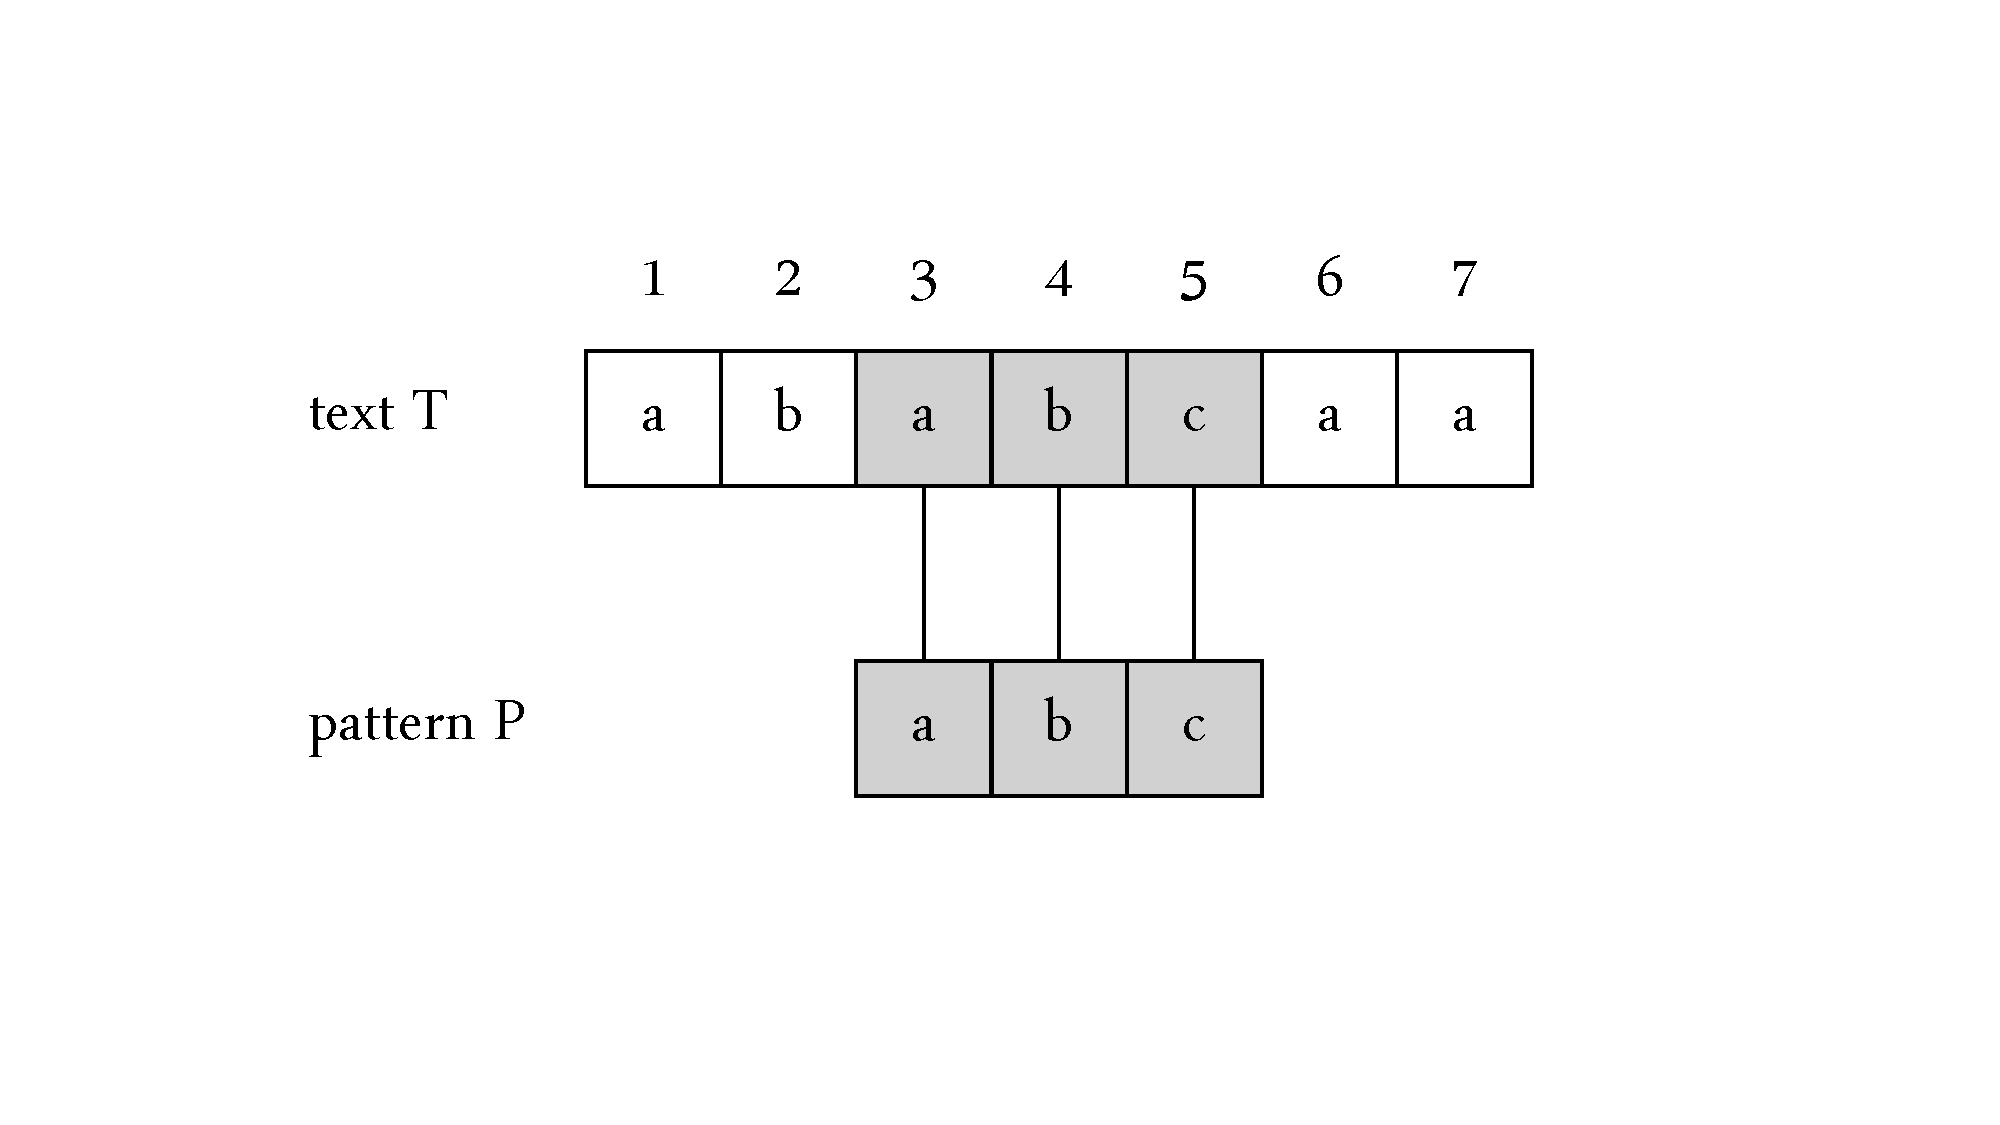
\includegraphics[width=0.8\textwidth, trim={2cm 5cm 2cm 3cm}, clip]{data/Illustrations/problem-statement1.pdf}
            \caption{T = "ababcab" and P = "abc"}
        \end{figure}
        \item If $T = \text{``aaaaa''}$ and $P = \text{``aa''}$, then the output is $(1 \rightarrow 2)$, $(2 \rightarrow 3)$, $(3 \rightarrow 4)$, and $(4 \rightarrow 5)$ because the pattern occurs at positions 1, 2, 3, and 4 in the text.
        \begin{figure}[h]
            \centering
            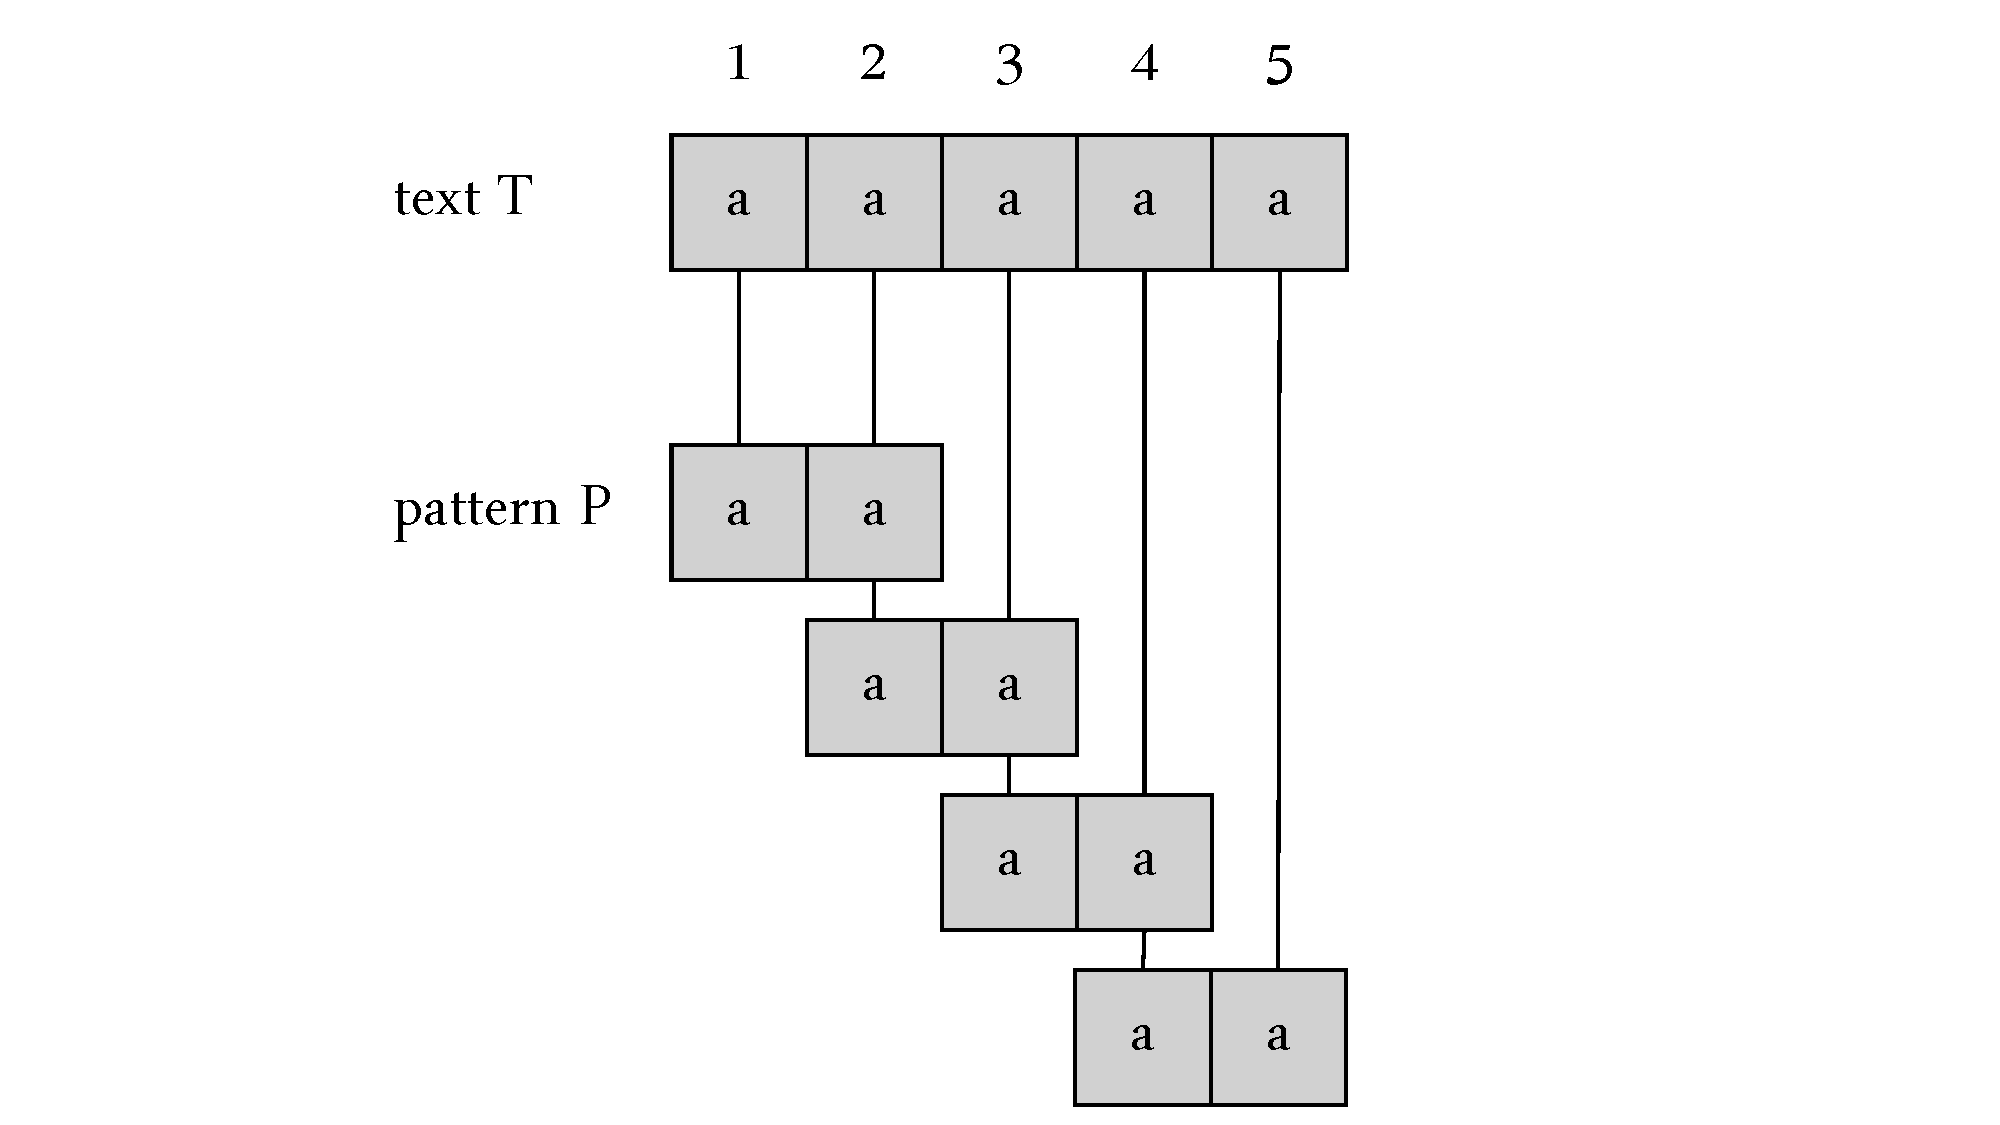
\includegraphics[width=0.8\textwidth, trim={2cm 0cm 2cm 0cm}, clip]{data/Illustrations/problem-statement2.pdf}
            \caption{T = "aaaaa" and P = "aa"}
        \end{figure}
    \end{itemize}